\chapter{Uncertainty, Time Evolution, and Spin Precession}

Susskind opens this lecture with a crowded agenda: uncertainty, more Schr\"odinger equation, time evolution, and finally the promised return to the single spin. He also pauses to remind us why the subject still feels abstract. Classical mechanics got from states to motion almost at once; quantum mechanics has taken a long preliminary climb. But the point of this lecture is that the climb is beginning to pay off. We first ask what it means for two observables to be sharp together, then we rebuild the logic of time evolution, and only after that do we let the formalism loose on a spin in a magnetic field. These notes follow that order and preserve the lecture's visual record through Leonard Susskind, LazyingArt LLC, and Video2Book.

\begin{figure}[ht]
\centering

\includegraphics[width=0.72\textwidth]{lecture_05_figure_01.png}
\caption{Opening title card. It carries no mathematics, but it is the lecture's first visual beat.}
\end{figure}

\section{Simultaneous Measurement, Common Eigenvectors, and Commutativity}

Susskind does not begin with the quantitative uncertainty principle. He begins with the more primitive question: what does it mean to measure something well? A good measurement must leave the system, at least momentarily, in a state for which the measured quantity is definite. Otherwise one could not immediately repeat the measurement and confirm the result.

\begin{definition}
An observable is represented by a Hermitian operator. Its possible measurement outcomes are its eigenvalues, and a state in which the observable has a definite value is an eigenvector of that operator.
\end{definition}

Now suppose that two observables can be simultaneously measured. Then a successful simultaneous measurement must leave the system in a state that is definite for both of them. That is the whole conceptual core of the argument.

\begin{remark}
Throughout this lecture Susskind uses the word basis in the physicist's sense: a complete orthonormal basis. He remarks that mathematicians use a broader notion, but orthonormality is the relevant notion here. If degeneracies occur, the eigenvectors are not unique, but they may be chosen orthonormal.
\end{remark}

Let us call the two observables \(L\) and \(M\). If they are simultaneously measurable, there must exist a complete orthonormal basis \(\{|i\rangle\}\) of simultaneous eigenvectors:
\begin{equation}
L|i\rangle = l_i|i\rangle,
\qquad
M|i\rangle = m_i|i\rangle.
\end{equation}
The lecture then proves the theorem in the most concrete possible way, by acting on a basis vector and comparing the two possible orders.

\begin{figure}[ht]
\centering

\includegraphics[width=0.82\textwidth]{lecture_05_figure_02.png}
\caption{\(ML\) and \(LM\) acting the same on the basis.}
\end{figure}

\begin{theorem}
If two observables can be simultaneously measured, then the corresponding Hermitian operators commute.
\end{theorem}

\begin{proof}
Act first with \(L\) and then with \(M\):
\begin{align}
ML|i\rangle
&= M\bigl(l_i|i\rangle\bigr) \\
&= l_i\,M|i\rangle \\
&= l_i m_i |i\rangle.
\end{align}
Now reverse the order:
\begin{align}
LM|i\rangle
&= L\bigl(m_i|i\rangle\bigr) \\
&= m_i\,L|i\rangle \\
&= m_i l_i |i\rangle \\
&= l_i m_i |i\rangle.
\end{align}
Thus \(ML\) and \(LM\) have the same action on every basis vector. Since any vector is a superposition of basis vectors, they have the same action on any vector. Therefore
\begin{equation}
[L,M]\equiv LM-ML=0.
\end{equation}
\end{proof}

The converse statement is also quoted in the lecture: if two Hermitian operators commute, then one can find a complete basis of simultaneous eigenvectors. That stronger direction is not reproved here, but it is the other half of the same theorem. In practice this is what makes simultaneously measurable quantities possible in the first place.

This abstract discussion immediately becomes concrete for spin. The operators \(\sigma_x\), \(\sigma_y\), and \(\sigma_z\) do not commute pairwise, so they cannot be simultaneously sharp. The eigenvectors of \(\sigma_z\) are up and down, the eigenvectors of \(\sigma_x\) are left and right, and they are not the same states. That is the qualitative content of uncertainty before any inequality is written down.

It is also worth keeping in mind one class of easy examples. When a system is composed of two independent subsystems, observables of one subsystem commute with observables of the other. That is why, for example, one may simultaneously measure the \(z\)-component of the first spin and the \(z\)-component of the second spin in a two-spin system.

\subsection{Question \& Answer}

\paragraph{Why must simultaneous measurements leave a common eigenbasis?}
A student asks for this point again, and Susskind's answer is operational. A measurement leaves the system in a state of definite thatness, meaning a state in which the measured quantity has a definite value. In our language, that means an eigenvector. If two observables can be measured simultaneously and both yield definite values, then the post-measurement state must be an eigenvector of both. Repeating this for the full set of possible outcomes leads to a complete common eigenbasis.

For a noncommuting pair such as \(\sigma_x\) and \(\sigma_z\), this cannot happen. One may measure either one, and after the measurement one may immediately repeat that same measurement and obtain the same answer. But one cannot make both quantities simultaneously definite. That is the first structural reason uncertainty exists at all.

\section{Recap of Time Evolution and the Emergence of the Hamiltonian}

Having made uncertainty concrete, Susskind deliberately resets the lecture. This is review, he says, but review with a purpose. He jokes that quantum mechanics has taken many pages to reach the point where classical mechanics had already started discussing motion. The good news is that once the state concept is in place, the rest begins to compress.

If the state at time \(0\) is \(|\psi(0)\rangle\), then the state at time \(t\) is obtained by a linear operator \(U(t)\):
\begin{equation}
|\psi(t)\rangle = U(t)|\psi(0)\rangle.
\end{equation}
The basic physical principle is conservation of distinctions: orthogonal states remain orthogonal under time evolution. If \(|i\rangle\) and \(|j\rangle\) are members of an orthonormal basis, then
\begin{equation}
\langle j|U^\dagger(t)U(t)|i\rangle = \delta_{ji}.
\end{equation}
Because this is true for every pair of basis vectors, it follows that
\begin{equation}
U^\dagger(t)U(t)=I.
\end{equation}
Thus the time-evolution operator is unitary.

Now take an infinitesimal time step \(\epsilon\). Continuity says that in a very short time the evolution operator should be very close to the identity. We therefore write
\begin{equation}
U(\epsilon)=I-i\epsilon H,
\qquad
U^\dagger(\epsilon)=I+i\epsilon H^\dagger.
\end{equation}
Susskind emphasizes that the factors of \(i\), \(\epsilon\), and even \(\hbar\) are partly a matter of convention at this stage; one could absorb them into the definition of \(H\). What matters is what unitarity then forces upon us. Substituting these expressions into \(U^\dagger U=I\) and keeping terms only through first order in \(\epsilon\), we find
\begin{equation}
H^\dagger=H.
\end{equation}

That is the decisive point. The generator of time evolution is Hermitian, and therefore it is an observable. This is why we identify \(H\) with the Hamiltonian, or energy operator.

One student asks whether orthogonality preservation is merely an empirical input. Susskind's answer is that it is empirical, but also extraordinarily rigid. In his language, quantum mechanics is brittle: if one tries to deform the rules slightly, positivity of probabilities or locality or some other essential feature quickly breaks. For present purposes, we simply take unitarity as the correct dynamical principle.

\begin{figure}[ht]
\centering

\includegraphics[width=0.82\textwidth]{lecture_05_figure_03.png}
\caption{Difference quotient for state evolution.}
\end{figure}

Now apply \(U(\epsilon)\) to the state:
\begin{equation}
|\psi(\epsilon)\rangle = |\psi(0)\rangle - i\epsilon H|\psi(0)\rangle.
\end{equation}
Move the initial state to the left and divide by \(\epsilon\). The board writes this as the visible difference quotient
\begin{equation}
\frac{|\psi(\epsilon)\rangle-|\psi(0)\rangle}{\epsilon}=-\,i\,H|\psi(0)\rangle.
\end{equation}
In the limit \(\epsilon\to 0\), the left-hand side becomes the time derivative of the state vector:
\begin{equation}
\frac{d}{dt}|\psi\rangle=-\,i\,H|\psi\rangle.
\end{equation}
This is the time-dependent Schr\"odinger equation.

Susskind pauses over its meaning. It sounds deterministic, and in one sense it is: if the system is left alone, the state evolves in a definite way. But that does not mean that the outcomes of all measurements are determined. The state tells us probabilities, not a list of pre-existing answers. So the Schr\"odinger equation is best understood as a rule for updating the state's probability content.

There is also a familiar caveat. This is the evolution of an undisturbed system. A measurement generally disturbs the system. The special exception is the case in which the system was already in an eigenstate of the observable being measured.

\section{Energy Eigenstates and the General Solution of Schr\"odinger Evolution}

At this point the lecture distinguishes the time-dependent Schr\"odinger equation from the time-independent one. Since \(H\) is Hermitian, it is itself an observable, and its eigenvalues are the possible outcomes of an energy measurement:
\begin{equation}
H|E_i\rangle = E_i|E_i\rangle.
\end{equation}
This is the time-independent Schr\"odinger equation.

The actual spectrum depends on the system: atoms have discrete levels, unbound motion may have a continuous spectrum, and so on. But the task is always the same. If we know \(H\), we solve its eigenvalue problem. Susskind then says: let us suppose that part has already been done. We know the eigenvectors and eigenvalues. The next question is how an arbitrary state evolves in time.

The board returns to the energy basis and identifies the generic basis vector \(|i\rangle\) with an energy eigenvector \(|E_i\rangle\).

\begin{figure}[ht]
\centering

\includegraphics[width=0.82\textwidth]{lecture_05_figure_05.png}
\caption{State expanded in energy eigenvectors.}
\end{figure}

The lower line in the screenshot is partly obscured, so here we use the standard reconstruction that matches the transcript:
\begin{equation}
|i\rangle = |E_i\rangle,
\qquad
|\psi(t)\rangle = \sum_j \alpha_j(t)\,|j\rangle.
\end{equation}
The states \(|j\rangle\) are fixed. The time dependence lies entirely in the coefficients \(\alpha_j(t)\).

The board derivation briefly gets tangled in its indices, and Susskind corrects himself in public. The cleaned calculation is straightforward. Differentiate the expansion:
\begin{equation}
\frac{d}{dt}|\psi(t)\rangle = \sum_j \dot{\alpha}_j(t)\,|j\rangle.
\end{equation}
On the other hand, Schr\"odinger's equation gives
\begin{align}
-\,iH|\psi(t)\rangle
&= -\,i \sum_j \alpha_j(t)\,H|j\rangle \\
&= -\,i \sum_j E_j\alpha_j(t)\,|j\rangle.
\end{align}
Since the same basis vectors appear on both sides, the corresponding coefficients must agree:
\begin{equation}
\dot{\alpha}_j(t)=-\,i\,E_j\,\alpha_j(t).
\end{equation}
Here \(j\) is fixed; there is no sum on \(j\) in this differential equation. For each energy eigencomponent we get a separate first-order equation, whose solution is
\begin{equation}
\alpha_j(t)=\alpha_j(0)e^{-iE_j t}.
\end{equation}
Substituting back into the expansion, we obtain the general solution of Schr\"odinger evolution:
\begin{equation}
|\psi(t)\rangle = \sum_j \alpha_j(0)e^{-iE_j t}|j\rangle.
\end{equation}

This is exactly the form Susskind wants us to remember. Take the initial state, decompose it into energy eigenvectors, and then let each component pick up its own phase. If the initial state happens already to be a single energy eigenstate, then only an overall phase appears:
\begin{equation}
|\psi(t)\rangle = e^{-iEt}|E\rangle.
\end{equation}
No measurable probability changes. The interesting time dependence arises only when more than one energy eigenstate is present.

Susskind also asks where \(\hbar\) would go if we restored it. The answer is in the denominator of the phase:
\begin{equation}
\alpha_j(t)=\alpha_j(0)e^{-iE_j t/\hbar}.
\end{equation}
This is the lecture's first direct connection between energy and oscillation. The magnitudes of the coefficients remain fixed:
\begin{equation}
|\alpha_j(t)|=|\alpha_j(0)|,
\end{equation}
and all the evolution is carried by relative phases.

\section{Expectation Values, Heisenberg Equations, and the Classical Analogy}

The next step is to shift attention from the state vector itself to averages of observables. Susskind complains, as he often does, that expectation value is not the best name; average would be better. But he uses the standard terminology anyway.

For an observable \(L\), the expectation value is
\begin{equation}
\langle L\rangle = \langle \psi|L|\psi\rangle.
\end{equation}
The state changes with time, so the expectation value changes with time. Differentiate:
\begin{align}
\frac{d}{dt}\langle L\rangle
&=
\frac{d}{dt}\langle \psi|L|\psi\rangle \\
&=
\langle \dot{\psi}|L|\psi\rangle + \langle \psi|L|\dot{\psi}\rangle.
\end{align}
Using the Schr\"odinger equation on the ket,
\begin{equation}
|\dot{\psi}\rangle = -iH|\psi\rangle,
\end{equation}
and the Hermitian-conjugate equation on the bra,
\begin{equation}
\langle \dot{\psi}| = i\langle \psi|H,
\end{equation}
we obtain
\begin{align}
\frac{d}{dt}\langle L\rangle
&=
i\langle \psi|HL|\psi\rangle - i\langle \psi|LH|\psi\rangle \\
&=
-\,i\,\langle \psi|(LH-HL)|\psi\rangle.
\end{align}

\begin{figure}[ht]
\centering

\includegraphics[width=0.82\textwidth]{lecture_05_figure_04.png}
\caption{Expectation values evolve by a commutator.}
\end{figure}

Thus the clean final equation is
\begin{equation}
\frac{d}{dt}\langle L\rangle = -\,i\,\langle [L,H]\rangle.
\end{equation}
Susskind sometimes abbreviates this as
\begin{equation}
\dot L = -\,i[L,H],
\end{equation}
but he is careful to warn that, at this stage, one should read this as shorthand for an equation about expectation values. The full Heisenberg-picture interpretation comes later.

We can also derive an explicit time-dependent matrix formula by inserting the energy-basis solution for the bra and ket:
\begin{align}
\langle L\rangle(t)
&=
\left(
\sum_k \alpha_k^*(0)e^{iE_k t}\langle k|
\right)
L
\left(
\sum_j \alpha_j(0)e^{-iE_j t}|j\rangle
\right) \\
&=
\sum_{k,j}\alpha_k^*(0)\alpha_j(0)e^{i(E_k-E_j)t}\langle k|L|j\rangle.
\end{align}
Defining the matrix elements
\begin{equation}
L_{kj}\equiv \langle k|L|j\rangle,
\end{equation}
this becomes
\begin{equation}
\langle L\rangle(t)=\sum_{k,j}\alpha_k^*(0)\alpha_j(0)e^{i(E_k-E_j)t}L_{kj}.
\end{equation}
This is the formula Susskind identifies with Heisenberg's matrix point of view: every matrix element carries a frequency difference \(E_k-E_j\).

\subsection{Question \& Answer}

\paragraph{Why does the factor \(i\) not make the time derivative imaginary?}
Susskind explicitly pauses over this. If \(\langle L\rangle\) is real, how can its time derivative be \(-i\) times something? His answer is not an abstract theorem first, but a promise: once we compute actual commutators of Hermitian observables, we will find that they come with explicit factors of \(i\). The extra \(i\) is waiting inside the commutator, so the final equation for real expectation values is itself real.

With that obstacle identified, the lecture steps back and studies the algebra of commutators. First, the commutator is odd:
\begin{equation}
[A,B]=-[B,A].
\end{equation}
Second, it satisfies the same product rule as the Poisson bracket.

\begin{proposition}
For operators \(A\), \(B\), and \(C\),
\begin{equation}
[AB,C]=A[B,C]+[A,C]B.
\end{equation}
\end{proposition}

\begin{proof}
Write out the commutator directly:
\begin{align}
[AB,C]
&=ABC-CAB.
\end{align}
Now add and subtract \(ACB\):
\begin{align}
[AB,C]
&=ABC-ACB+ACB-CAB \\
&=A(BC-CB)+(AC-CA)B \\
&=A[B,C]+[A,C]B.
\end{align}
\end{proof}

This is exactly the kind of algebraic rule that Poisson brackets satisfy in classical mechanics. That is not an accident. In the units used through most of the lecture, \(\hbar=1\), and the structural correspondence is
\begin{equation}
\{L,H\}\leftrightarrow -\,i[L,H].
\end{equation}
If we restore \(\hbar\), then the dimensionful form is
\begin{equation}
\{L,H\}\leftrightarrow -\,\frac{i}{\hbar}[L,H].
\end{equation}
This is why \(H\) deserves the name Hamiltonian. In classical mechanics one writes
\begin{equation}
\frac{dL}{dt}=\{L,H\},
\end{equation}
and in quantum mechanics, in the sense of averages, the corresponding rule is
\begin{equation}
\frac{d}{dt}\langle L\rangle=-\,i\,\langle [L,H]\rangle.
\end{equation}
Here \(L\) is any observable, not specifically angular momentum.

The simplest application is to take \(L=H\):
\begin{equation}
\frac{d}{dt}\langle H\rangle = -\,i\,\langle [H,H]\rangle = 0.
\end{equation}
So the average energy is conserved. Susskind remarks that quantum mechanics says something even stronger, but not tonight.

\section{A Single Spin in a Magnetic Field}

Only now, after all this apparatus, does the lecture return to the single spin. A student asks: what is \(H\) for a spin? Susskind's answer is that a free isolated spin has no interesting Hamiltonian, at least up to an additive constant. The dynamics becomes nontrivial only when the spin interacts with something, and the simplest interaction is with a magnetic field.

Take the magnetic field along the \(z\)-axis.

\begin{figure}[ht]
\centering

\includegraphics[width=0.86\textwidth]{lecture_05_figure_06.png}
\caption{Magnetic field along \(z\) and spin Hamiltonian setup.}
\end{figure}

\begin{figure}[ht]
\centering
\begin{tikzpicture}[scale=1.15]
\draw[->] (0,0) -- (0,2.7) node[above] {$B_z$};
\draw[->] (0.3,0.3) -- (1.7,1.6);
\draw (3.3,1.35) node {$H=\dfrac{\omega}{2}\sigma_z$};
\end{tikzpicture}
\caption{A clean redraw of the board sketch: field along \(z\), with a tilted spin direction shown only as a mnemonic.}
\end{figure}

Susskind is careful here. The sketch is suggestive, but it must not be taken literally. A spin is not really a little arrow that one can draw in classical space. In fact he jokes that this is why quantum books have fewer figures than classical mechanics books: the things we are talking about cannot all be made simultaneously pictorial. Still, the sketch helps us remember the direction of the field.

The physical guess is familiar from classical magnetism. A magnetic dipole in a magnetic field has an energy proportional to the dot product of the dipole with the field. If the field is along \(z\), the Hamiltonian should therefore be proportional to the \(z\)-component of spin:
\begin{equation}
H=\frac{\omega}{2}\sigma_z.
\end{equation}
The coefficient \(\omega/2\) absorbs the magnetic moment, the field strength, and the other constants. Susskind says explicitly that the reason for both the symbol \(\omega\) and the factor of \(2\) will become clear shortly.

The spin components are represented by the Pauli matrices,
\begin{equation}
\sigma_x=
\begin{pmatrix}
0&1\\
1&0
\end{pmatrix},
\qquad
\sigma_y=
\begin{pmatrix}
0&-i\\
i&0
\end{pmatrix},
\qquad
\sigma_z=
\begin{pmatrix}
1&0\\
0&-1
\end{pmatrix}.
\end{equation}
What we want are the equations of motion for the averages of \(\sigma_x\), \(\sigma_y\), and \(\sigma_z\):
\begin{align}
\frac{d}{dt}\langle \sigma_x\rangle
&=
-\,i\left\langle\left[\sigma_x,\frac{\omega}{2}\sigma_z\right]\right\rangle, \\
\frac{d}{dt}\langle \sigma_y\rangle
&=
-\,i\left\langle\left[\sigma_y,\frac{\omega}{2}\sigma_z\right]\right\rangle, \\
\frac{d}{dt}\langle \sigma_z\rangle
&=
-\,i\left\langle\left[\sigma_z,\frac{\omega}{2}\sigma_z\right]\right\rangle.
\end{align}
The last equation is immediate:
\begin{equation}
\frac{d}{dt}\langle \sigma_z\rangle = 0.
\end{equation}
So the component of spin along the field is conserved.

To go further we need the commutation relations of the Pauli matrices. Susskind computes them by matrix multiplication. For example,
\begin{align}
[\sigma_z,\sigma_x]
&=
\begin{pmatrix}
1&0\\
0&-1
\end{pmatrix}
\begin{pmatrix}
0&1\\
1&0
\end{pmatrix}
-
\begin{pmatrix}
0&1\\
1&0
\end{pmatrix}
\begin{pmatrix}
1&0\\
0&-1
\end{pmatrix} \\
&=
\begin{pmatrix}
0&1\\
-1&0
\end{pmatrix}
-
\begin{pmatrix}
0&-1\\
1&0
\end{pmatrix} \\
&=
2
\begin{pmatrix}
0&1\\
-1&0
\end{pmatrix}
=
2i\sigma_y.
\end{align}
The other commutators follow by cyclic permutation:
\begin{equation}
[\sigma_z,\sigma_x]=2i\sigma_y,
\qquad
[\sigma_x,\sigma_y]=2i\sigma_z,
\qquad
[\sigma_y,\sigma_z]=2i\sigma_x.
\end{equation}
If we reverse the order of any commutator, the sign changes. Thus
\begin{equation}
[\sigma_x,\sigma_z]=-2i\sigma_y.
\end{equation}

Now the earlier puzzle about the factor of \(i\) resolves itself exactly as promised:
\begin{align}
\frac{d}{dt}\langle \sigma_x\rangle
&=
-\,i\,\frac{\omega}{2}\langle[\sigma_x,\sigma_z]\rangle \\
&=
-\,i\,\frac{\omega}{2}\langle-2i\sigma_y\rangle \\
&=
-\omega\langle \sigma_y\rangle,
\end{align}
and similarly,
\begin{align}
\frac{d}{dt}\langle \sigma_y\rangle
&=
-\,i\,\frac{\omega}{2}\langle[\sigma_y,\sigma_z]\rangle \\
&=
-\,i\,\frac{\omega}{2}\langle 2i\sigma_x\rangle \\
&=
+\omega\langle \sigma_x\rangle.
\end{align}
Collecting the three equations, we have
\begin{equation}
\dot{\langle \sigma_x\rangle}=-\omega\langle \sigma_y\rangle,
\qquad
\dot{\langle \sigma_y\rangle}=+\omega\langle \sigma_x\rangle,
\qquad
\dot{\langle \sigma_z\rangle}=0.
\end{equation}

\begin{figure}[ht]
\centering
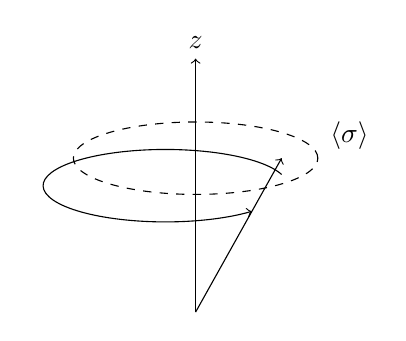
\begin{tikzpicture}[scale=1.15]
\draw[->] (0,0) -- (0,2.8) node[above] {$z$};
\draw[dashed] (0,1.7) ellipse (1.35 and 0.4);
\draw[->] (0,0) -- (0.95,1.7);
\draw[->] (0.95,1.52) arc[start angle=18,end angle=315,x radius=1.35,y radius=0.4];
\draw (1.7,1.95) node {$\langle \sigma\rangle$};
\end{tikzpicture}
\caption{The mathematical consequence of the equations of motion: the expectation-value vector precesses about the field axis.}
\end{figure}

These are exactly the equations of circular motion. In the sense of expectation values, the spin precesses about the \(z\)-axis, just as a classical rotor or gyroscope would in a magnetic field. Susskind is very explicit about the sense in which this is true. The operators themselves do not literally move in space. What changes with time is the state, and therefore the expectation values of the spin components.

\section{General Field Direction and Closing Clarifications}

A natural question now arises: why was \(H=\omega\sigma_z/2\) the right guess? Susskind answers by pointing out how little room there is in a two-dimensional state space. The most general Hermitian \(2\times2\) operator is
\begin{equation}
H=aI+b_x\sigma_x+b_y\sigma_y+b_z\sigma_z.
\end{equation}
The identity term is dynamically uninteresting. It merely adds a constant to the energy, and constants commute with everything. So the nontrivial part of the Hamiltonian is always some linear combination of the three Pauli matrices.

That is exactly what one would expect for a magnetic field pointing in a general direction. If the field points along a unit vector \(n\), then the natural Hamiltonian is
\begin{equation}
H=\frac{\omega}{2}\,\sigma\cdot n,
\qquad
\sigma\cdot n \equiv n_x\sigma_x+n_y\sigma_y+n_z\sigma_z.
\end{equation}
Here \(\sigma\cdot n\) is matrix shorthand. It is not literally a classical vector dot product, but a compact way of naming a single \(2\times2\) matrix. If we write out that matrix, we get
\begin{equation}
\sigma\cdot n=
\begin{pmatrix}
n_z & n_x-i n_y \\
n_x+i n_y & -n_z
\end{pmatrix}.
\end{equation}
The relation to the magnetic field is
\begin{equation}
\mathbf{B}=B\,\mathbf{n},
\end{equation}
so \(n\) carries the direction and \(\omega\) carries the overall scale.

Susskind then asks for the eigenvalues of \(\sigma\cdot n\). If \(n\) is a unit vector, then
\begin{equation}
n_x^2+n_y^2+n_z^2=1.
\end{equation}
Let the two eigenvalues be \(\lambda_1\) and \(\lambda_2\). The trace is zero, so
\begin{equation}
\lambda_1+\lambda_2=0.
\end{equation}
The determinant is
\begin{equation}
\det(\sigma\cdot n)=-(n_x^2+n_y^2+n_z^2)=-1,
\end{equation}
so
\begin{equation}
\lambda_1\lambda_2=-1.
\end{equation}
The only pair of numbers satisfying both conditions is
\begin{equation}
\lambda_\pm=\pm 1.
\end{equation}
Therefore the energies of the Hamiltonian \(H=\frac{\omega}{2}\sigma\cdot n\) are always
\begin{equation}
E_\pm=\pm \frac{\omega}{2},
\end{equation}
and the energy gap is
\begin{equation}
\Delta E=\omega.
\end{equation}
This is independent of the direction of the field. What changes with the direction is which component of spin is conserved. For a field along \(n\), the component of spin along \(n\) stays fixed, while the perpendicular components precess around that axis.

\subsection{Question \& Answer}

\paragraph{How can a two-dimensional state space give a three-dimensional precession picture?}
The lecture lingers on this because it is exactly where classical intuition starts to mislead. The space of states for a single spin is two-dimensional. The three-dimensional object we draw or talk about is not the state vector itself; it is the triple of expectation values \((\langle \sigma_x\rangle,\langle \sigma_y\rangle,\langle \sigma_z\rangle)\). These live in ordinary space and behave like the components of a real vector. They are related to the state, but they are not the same thing.

\paragraph{Why is the magnetic field not treated as an operator?}
Because, for the purposes of this lecture, the magnet is regarded as part of a heavy apparatus. If we included the magnet as part of the full quantum system, then the field would arise from a larger quantum-mechanical problem. But when a system is large, heavy, and only weakly affected by the electron, its fluctuations are negligible and we treat it as classical. Susskind stresses that this division between quantum system and classical apparatus is only provisional. One must eventually justify it. But not tonight.

\paragraph{Are these equations exact for a single run, or only for averages?}
Only for averages. The equations
\begin{equation}
\dot{\langle \sigma_x\rangle}=-\omega\langle \sigma_y\rangle,
\qquad
\dot{\langle \sigma_y\rangle}=+\omega\langle \sigma_x\rangle,
\qquad
\dot{\langle \sigma_z\rangle}=0
\end{equation}
describe what repeated experiments average to. A single trial need not follow this smooth precessional story. Susskind says quite plainly that the bridge from probability distributions to laboratory averages is a basic postulate of statistical reasoning, not something he intends to justify here.

\paragraph{What happens for a sideways spin? Does it emit half a photon?}
No. This is the lecture's last important clarification. A spin whose expectation value points sideways is not in a single energy eigenstate. It is in a superposition of the up and down energy states. Therefore it does not emit half the energy gap. Instead there is some probability that it emits a full photon of energy \(\omega\), and some probability that it emits nothing. In the symmetric case, the probability to emit is one half, so the average emitted energy is half of \(\omega\), but each individual emission event still carries the full quantum \(\omega\).

\paragraph{What does \(\omega\) measure?}
\(\omega\) is just a number. Up to the lecture's conventions, it is proportional to the magnitude of the magnetic field times the magnetic moment of the spin. It does not know the direction of the field. The direction is carried by \(n\), while \(\omega\) sets the energy splitting and therefore the precession frequency.

\section{Summary}

This lecture turns abstract principles into motion. A good measurement leaves a system in an eigenstate, and from that simple idea we learned why simultaneous measurability leads to commuting observables. The noncommutation of the Pauli matrices then gave the first qualitative glimpse of uncertainty. From there Susskind deliberately reset the story and rebuilt the dynamics: unitarity implied a Hermitian generator \(H\), infinitesimal evolution produced the time-dependent Schr\"odinger equation, and diagonalizing \(H\) gave the general solution in the energy basis. Expectation values were then shown to evolve by commutators, revealing the quantum analog of Hamilton's equations. Finally, when the Hamiltonian was chosen for a spin in a magnetic field, all the formalism paid off at once: the expectation values of the spin components precess about the field direction, the component along the field remains fixed, and the general Hamiltonian \(\frac{\omega}{2}\sigma\cdot n\) makes clear that this is the most general nontrivial dynamics a single spin can have.